\section{\sys\ Design}
\label{sec:design}



This section presents the design challenges of building a hardware-based \md\ system and our solutions.
%, including a hardware-based virtual memory system
%and a network system.
%, and framework for computation offloading.

\subsection{Design Challenges and Principles}
Building a hardware-based \md\ platform is a previously unexplored area and introduces new challenges mainly because of restrictions of hardware and the unique requirements of \md.
%Below, we discuss these challenges and our design principles.


\boldpara{Challenge 1: The hardware should avoid maintaining or processing complex data structures}, because unlike software, hardware has limited resources such as on-chip memory and logic cells.
For example, Linux and many other software systems use trees (\eg, the vma tree) for allocation.
Maintaining and searching a big tree data structure in hardware, however, would require huge on-chip memory and many logic cells to perform the look up operation (or alternatively use fewer resources but suffer from performance loss).


\boldpara{Challenge 2: Data buffers and metadata that the hardware uses should be minimal and have bounded sizes}, so that they can be statically planned and fit into the on-chip memory.
Unfortunately, traditional software approaches 
% (usually unawaringly) 
involve various data buffers and metadata that are large and grow with increasing scale.
%; they thus cannot meet our goal.
For example, today's reliable network transports maintain per-connection sequence numbers and buffer unacknowledged packets for packet ordering and retransmission, and they grow with the number of connections.
Although swapping between on-chip and off-chip memory is possible, doing so would increase both tail latency and hardware logic complexity, especially under large scale.
%Thus, it is desirable to resort as little as possible to swapping. 
%Achieving the bounded buffer/state goal is even harder when we simultaneously need to meet our scalability goals.


\boldpara{Challenge 3: The hardware pipeline should be deterministic and smooth},
\ie, it uses a bounded, known number of cycles to process a data unit, and for each cycle, the pipeline can take in one new data unit (from the network).
The former would ensure low tail latency, while the latter would guarantee a throughput that could match network line rate.
Another subtle benefit of a deterministic pipeline is that we can know the maximum time a data unit stays at \MN,
which could help bound the size of certain buffers (\eg, \S\ref{sec:ordering}).
%\md's low latency and low tail latency requirements (\textbf{R3} and \textbf{R4})
However, many traditional hardware solutions are not designed to be deterministic or smooth, and we cannot directly adapt their approaches.
For example, traditional CPU pipelines could have stalls because of data hazards and have non-deterministic latency to handle memory instructions.
%in a traditional in-order CPU pipeline, stalls can happen because of data hazards such as read-after-write (RAW);
%out-of-order pipelines avoid such stalls but are too complex to implement in a small device like \hdm.
%This means that we need to seek other ways to deliver our guaranteed read/write dependencies (\$\ref{sec:ordering}).

To confront these challenges, we took a clean-slate approach by designing \sys's virtual memory system and network system with the following principles that all aim to eliminate state in hardware or bound their performance and space overhead.

\boldpara{Principle 1: Avoid state whenever possible.}
Not all state in server-based solutions is necessary if we could redesign the hardware.
For example, we get rid of RDMA's MR indirection and its metadata altogether
by directly mapping application process' \rspace\ VAs to PAs (instead of to MRs then to PAs).
%Another type of states that we get rid of is network connections.

\boldpara{Principle 2: Moving non-critical operations and state to software and making the hardware fast path deterministic.}
If an operation is non-critical and it involves complex processing logic and/or metadata, our idea is to move it to the software slow path running in an ARM processor.
For example, VA allocation (\alloc) is expected to be a rare operation
because applications know the disaggregated nature and would typically have only a few large allocations during the execution.
Handling \alloc, however, would involve dealing with complex allocation trees.
We thus handle \alloc\ and \sysfree\ in the software slow path.
Furthermore, in order to make the fast path performance deterministic, we {\em decouple} all slow-path tasks from the performance-critical path by {\em asynchronously} performing them in the background.
%Note that page fault is a relatively critical operation, as all first accesses to allocated virtual pages will cause a fault, and applications like serverless computing could access large amounts of (new) memory in a short period of time.



\boldpara{Principle 3: Shifting functionalities and state to \CN{}s.}
While hardware resources are scarce at \MN{}s, \CN{}s have sufficient memory and processing power, and it is faster to develop functionalities in \CN\ software.
A viable solution is to shift state and functionalities from \MN{}s to \CN{}s.
The key question here is how much and what to shift.
%; shifting too much would make \sys\ similar to \pdm\ and suffer from various performance and security issues of \pdm.
Our strategy is to shift functionalities to \CN{}s only if doing so 1) could largely reduce hardware resource consumption at \MN{}s, 2) does not slow down common-case foreground data operations, 3) does not sacrifice security guarantees, and 4) adds bounded memory space and CPU cycle overheads to \CN{}s.
As a tradeoff, the shift may result in certain uncommon operations (\eg, handling a failed request) being slower.
%Our insight here is that we can if a shift results in performance tradeoff only for uncommon cases
%For example, traditional reliable network stacks require maintaining 

\boldpara{Principle 4: Making off-chip data structures efficient and scalable.}
Principles 1 to 3 allow us to reduce \MN\ hardware to only the most essential functionalities and state. 
We store the remaining state in off-chip memory and cache a fixed amount of them in on-chip memory.
Different from most caching solutions, our focus is to make the access to off-chip data structure fast and scalable,
\ie, all cache misses have bounded latency regardless of the number of client processes accessing an \MN\ or the amount of physical memory the \MN\ hosts.

\if 0
\boldpara{Principle 5: Making the hardware fast path deterministic by decoupling the slow path.}
A hardware pipeline can only be deterministic if every step in it is deterministic.
However, certain complex functionalities in our fast path have to use the assistance from the software slow path.
To avoid waiting for the slow path, our idea is to decouple it by {\em asynchronously} performing the slow-path tasks.
\fi

\boldpara{Principle 5: Making the hardware fast path smooth by treating each data unit independently at \MN.}
If data units have dependencies (\eg, must be executed in a certain order), then the fast path cannot always execute a data unit when receiving it.
To handle one data unit per cycle and reach network line rate, we make each data unit independent by including all the information needed to process a unit in it and by allowing \MN{}s to execute data units in any order that they arrive.
%there is no dependency check across data units at \MN{}s.
To deliver our consistency guarantees, we opt for enforcing request ordering at \CN{}s before sending them out.

The rest of this section presents how we follow these principles to design \sys's three main functionalities: memory address translation and protection, page fault handling, and networking. We also briefly discuss our offloading support.

\subsection{Scalable, Fast Address Translation}
\label{sec:addr-trans}
%Similar to traditional virtual memory addressing, we use fix-size pages as VA/PA allocation and address translation unit, while data accesses are in the unit of byte.
Similar to traditional virtual memory systems, we use fix-size pages as address allocation and translation unit, while data accesses are in the granularity of byte.
Despite the similarity in the goal of address translation,
%(\ie, translating a virtual page to a physical page number),
the radix-tree-style, per-address space page table design used by all current architectures~\cite{ecuckoo-asplos20} does not fit \md\ for two reasons.
First, each request from the network could be from a different client process. If each process has its own page table, \MN\ would need to cache and look up many page table roots, causing additional overhead.
Second, a multi-level page table design requires multiple DRAM accesses when there is a translation lookaside buffer (TLB) miss~\cite{hashpgtable-sigmetrics16}.
TLB misses will be much more common in a \md\ environment, since with more applications sharing an \MN, the total working set size is much bigger than that in a single-server setting, while the TLB size in an \MN\ will be similar or even smaller than a single server's TLB (for cost concerns). To make matters worse, each DRAM access is more costly for systems like RDMA NIC which has to cross the PCIe bus to access the page table in main memory~\cite{Pythia,pcie-sigcomm}.
%\yiying{Can we add that paper's reference on RDMA's perf is multiple times worse with TLB miss?} 
%, increasing the tail latency of \md.
%and requires an additional lookup to identify the location of the page table root.
%Third, page table size grows with the number of processes and the allocated VA addresses, even though not all of them are used.
%Together, they affect the median latency, tail latency, and scalability when used for \md.

\ulinebfpara{Flat, single page table design (Principle 4).}~~
We propose a new {\em overflow-free} hash-based page table design that sets the total page table size according to the physical memory size 
and bounds \textit{address translation to at most one DRAM access}.
Specifically, we store {\em all} page table entries (PTEs) from {\em all} processes in a single hash table 
whose size is proportional to the physical memory size of an \MN. 
The location of this page table is fixed in the off-chip DRAM and is known by the fast path address translation unit, thus avoiding any lookups.
%We create the page table to always have enough entries to cover the entire physical memory.
As we anticipate applications to allocate big chunks of VAs in their \rspace, we use huge pages and support a configurable set of page sizes.
%Each PTE is 8 bytes, 
With the default 4\MB\ page size, the hash table consumes only 0.4\%\ of the physical memory.
%For example, for 1\TB\ physical memory and 4\MB\ page size, the whole page table is only 4\MB\ (each PTE is 8 bytes).

{
\begin{figure*}[th]
\begin{center}
\centerline{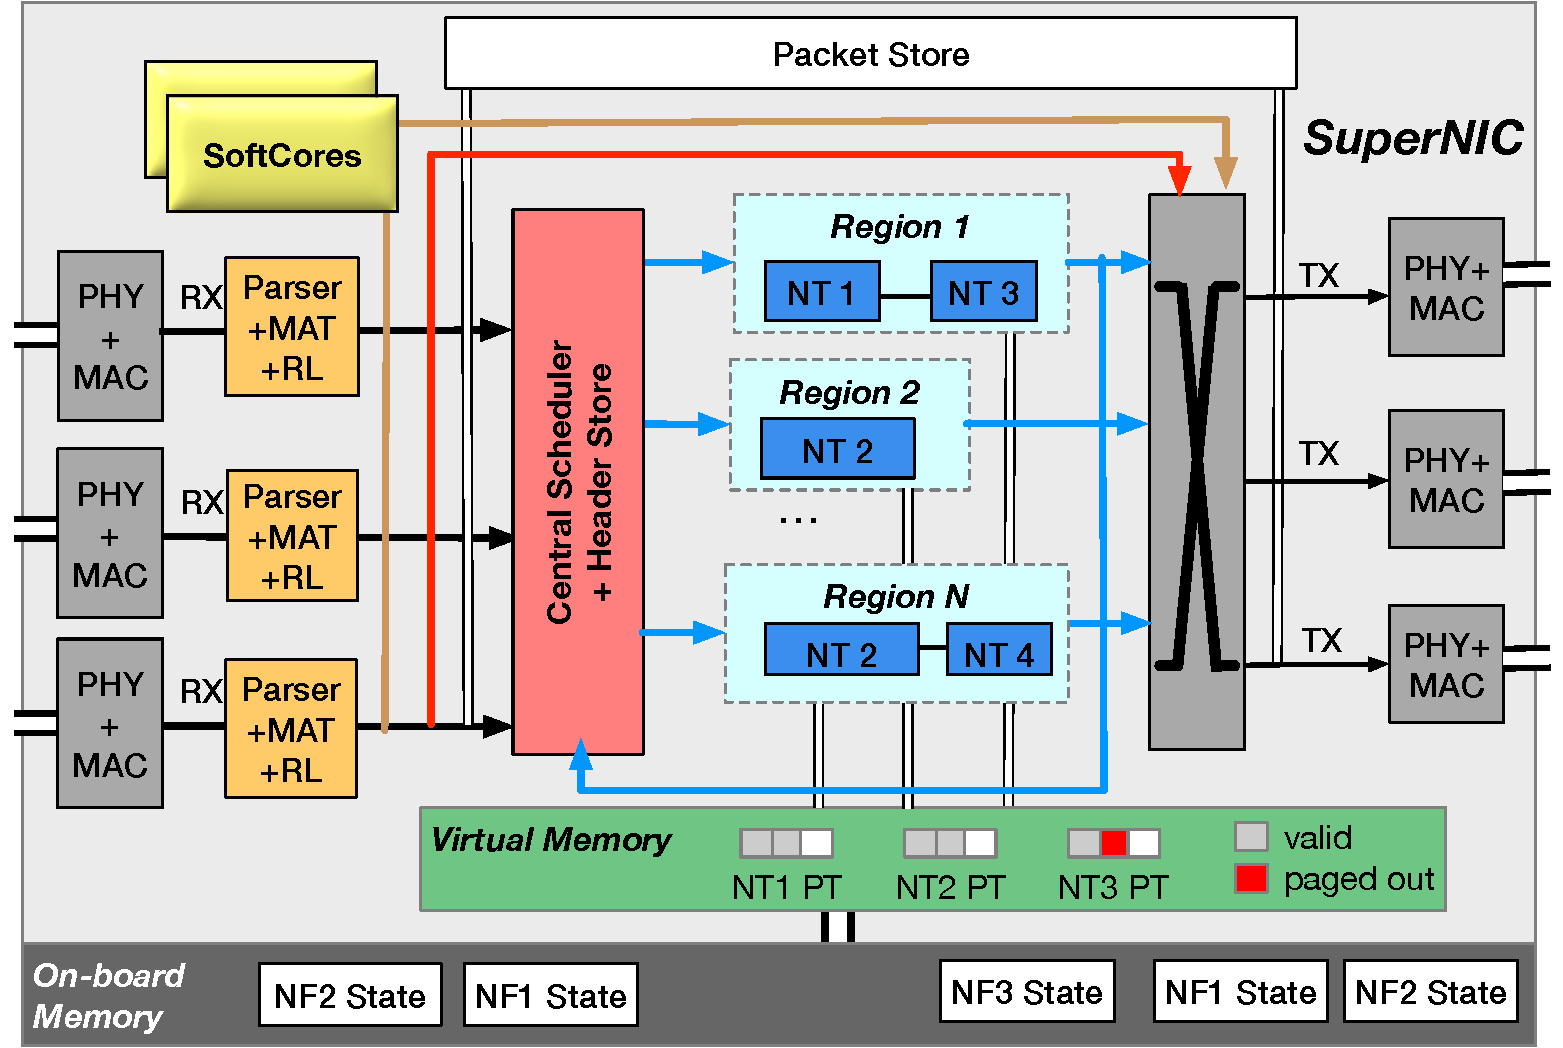
\includegraphics[width=\textwidth]{snic/Figures/board.pdf}}
\mycaption{fig-snic-board}{\snic\ On-Board Design.}
{
RL: Rate Limiter. PT: Page Table
}
\end{center}
\end{figure*}
}
{
\begin{figure*}[th]
\begin{center}
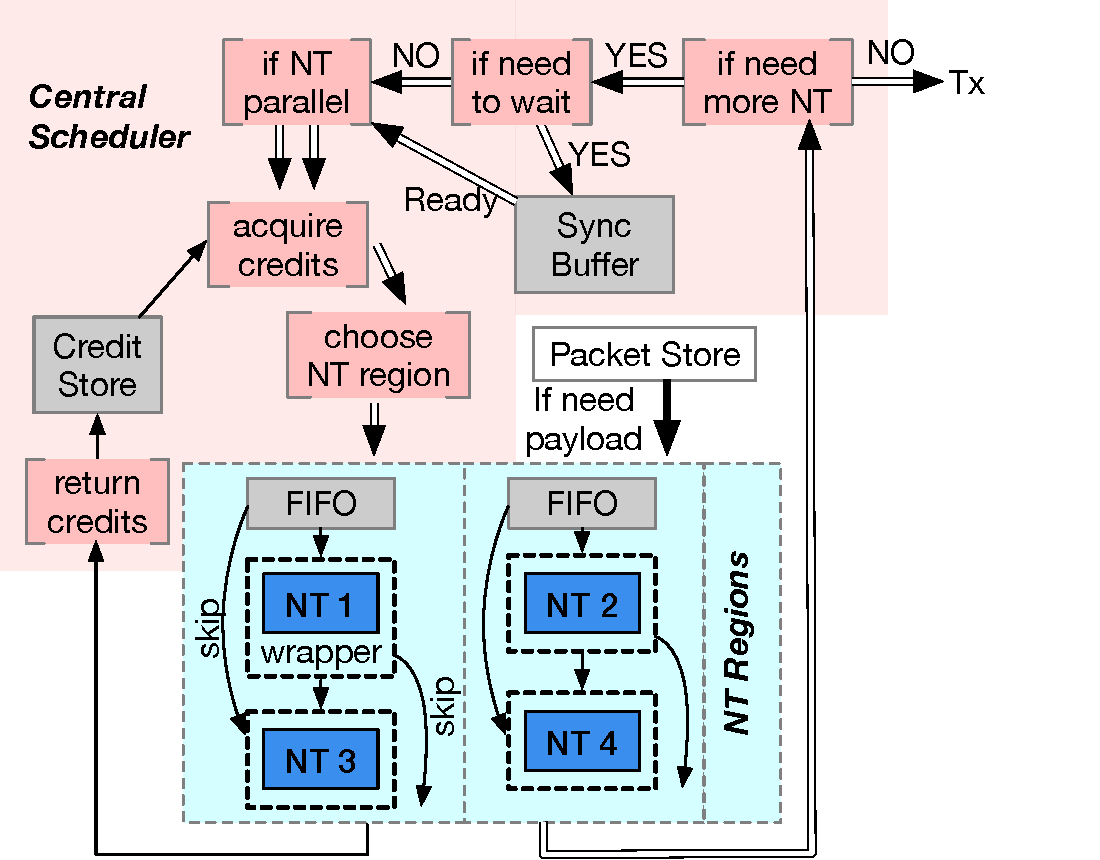
\includegraphics[width=0.9\textwidth]{snic/Figures/scheduler.pdf}
\mycaption{fig-sched}{\snic\ Packet Scheduler and \nt\ Region Design.}
{
Double arrows, single arrows, and thick arrows represent packet headers, credits, and packet payload.
}
\end{center}
\end{figure*}
}

The hash value of a VA and its PID is used as the index to determine which hash bucket the corresponding PTE goes to.
Each hash bucket has a fixed number of ($K$) slots.
To access the page table, we always fetch
the entire bucket including all $K$ slots in a single DRAM access.
%Normally, a hash table with fixed slots will have an overflow problem because of hash conflicts (\eg, when more than $K$ VA+PID combinations have the same hash value).

A well-known problem with hash-based page table design is hash collisions that could overflow a bucket.
Existing hash-based page table designs rely on collision chaining~\cite{TransCache-isca10} or open addressing~\cite{hashpgtable-sigmetrics16} to handle overflows, both require multiple DRAM accesses or even costly software intervention.
In order to bound address translation to at most one DRAM access, we use a novel technique to avoid hash overflows at \textit{VA allocation time}.

\ulinebfpara{VA allocation (Principle 2).}~~
The slow path software handles \alloc\ requests and allocates VA.
The software allocator maintains a per-process VA allocation tree that records allocated VA ranges and permissions, similar to the Linux vma tree~\cite{linux-rb-vma}.
To allocate size $k$ of VAs, it first finds an available address range of size $k$ in the tree.
It then calculates the hash values of the virtual pages in this address range
and checks if inserting them to the page table would cause any hash overflow. 
If so, it %marks the failed virtual pages in the tree as ``unusable'' and 
does another search for available VAs.
These steps repeat until it finds a valid VA range that does not cause hash overflow.
%It then send these VA page numbers (VPN) to the hardware fast path, which inserts the corresponding PTEs (invalid PTEs without PAs) to the page table. The last step is crucial for fast page fault handling in the hardware.
%It then send these VA page numbers and their permissions to the hardware fast path, which establishes the corresponding PTEs (with invalid state, \ie, with permission set up but no PAs). %The last step is crucial for fast page fault handling in the hardware as it enables in-line VA permission checking.

Our design trades potential retry overhead at allocation time (at the slow path) for better run-time performance and simpler hardware design (at the fast path).
% core-memory implementation.
This overhead is manageable because
1) each retry takes only a few microseconds with our implementation (\S\ref{sec:impl}),
%is fast even when running at ARM processor (\mus\ level), 
2) we employ huge pages, which means fewer pages need to be allocated, 
3) we choose a hash function that has very low collision rate~\cite{lookup3-wiki},
and 4) we set the page table to have extra slots (2\x\ by default) which absorbs most overflows.
%and 5) the \sys\ 64-bit virtual address space is huge.
%In fact, none of our evaluated application's \alloc\ requests ever require retry, even when the \alloc\ size is as huge as 1\TB.
We find no conflicts when memory is below half utilized and has only up to 60 retries when memory is close to full (Figure~\ref{fig-alloc-conflict}).

\ulinebfpara{TLB.}~~
%and its consistency with the page table.}
\sys\ implements a TLB in a fix-sized on-chip memory area and looks it up using content-addressable-memory in the fast path.
%and use LRU for replacement, 
On a TLB miss, the fast path fetches the PTE from off-chip memory and inserts it to the TLB by replacing an existing TLB entry with the LRU policy.
When updating a PTE, the fast path also updates the TLB, in a way that ensures the consistency of inflight operations.
%
%As with traditional TLB, \sys\ also faces a consistency problem between TLB and the page table.
%Traditionally, the OS needs to shootdown TLBs after modifying PTEs~\cite{tlbshootdown-eurosys20}.
%\sys's software slow path is the party that modifies a PTE, \eg, deleting a PTE when handling \sysfree.
%With our separate fast- and slow-path design, there could be potential %consistency problems when both paths try to access/modify the page table.
%The first consistency problem happens when the slow path needs to update the %page table (\eg, when handling a \sysfree).
%between slow-path generated PTE changes (update or delete) and fast-path TLB.
%Instead of letting the slow path change the page table in DRAM and shootdown the TLB in the on-chip memory,
%we let the hardware fast path pipeline handle all page table {\em and} TLB modifications.
%With the latter, it is easier to ensure the consistency of inflight fast-path operations, as they are in the same pipeline as the TLB/page-table modification logic.
%\zhiyuan{Is the above correct?}
%If it directly applies the change to the page table in DRAM, then the TLB will be inconsistent.
%Today's computer relies on the OS to perform costly~\cite{XXX} TLB shootdowns for TLB consistency.
%Following our design of only having the fast path managing TLB,
%To solve this problem, we adopt a simple principle: the fast path is the only unit accessing and changing TLB {\em and} the page table.
%We use a different approach where
%Thus, the slow path hands over its PTE change requests to the fast path, 
%which performs both the TLB change and the PTE change in its pipeline in a way that is consistent for inflight fast-path operations.

\ulinebfpara{Limitation.}~~
A downside of our overflow-free VA allocation design is that it cannot guarantee that a specific VA can be inserted into the page table. This is not a problem for regular VA allocation but could be problematic for allocations that require a fixed VA (\eg, \texttt{mmap(MAP\_FIXED})). 
Currently, \sys\ finds a new VA range if the user-specified range cannot be inserted into the page table. Applications that must map at fixed VAs (\eg, libraries) will need to use \CN-local memory.
%This semantics is the same as Linux \texttt{mmap(MAP\_FIXED\_NOREPLACE)}~\cite{linux-mmap-man}.
%Since we prevent hash overflow at VA allocation, fixed address allocation request may fail. This semantic is similar to \texttt{mmap(MAP\_FIXED\_NOREPLACE)}, both may return an address different from the requested one.
%2) a single global hash table needs extra software to track page sharing among processes~\cite{ecuckoo-asplos20}. We leave this for future work when we extend to a larger distributed setting.

\subsection{Low-Tail-Latency Page Fault Handling}

A key reason to disaggregate memory is to consolidate memory usages on less DRAM so that memory utilization is higher and the total monetary cost is lower (\textbf{R1}). Thus, remote memory space is desired to run close to full capacity, and we allow memory over-commitment at an \MN, necessitating page fault handling. Meanwhile, applications like JVM-based ones allocate a large heap memory space at the startup time and then slowly use it to allocate smaller objects~\cite{ali-trace}. Similarly, many existing far-memory systems~\cite{Tsai20-ATC,AIFM,FaRM} allocate a big chunk of remote memory and then use different parts of it for smaller objects to avoid frequently triggering the slow remote allocation operation.
In these cases, it is desirable for a \md\ system to delay the allocation of physical memory to when the memory is actually used (\ie, {\em on-demand} allocation) or to ``reshape'' memory~\cite{cliquemap-sigcomm21} during runtime, necessitating page fault handling.

Page faults are traditionally signaled by the hardware and handled by the OS. %, and they can happen when a PTE is invalid (VA created, PA not allocated)
%or when there is a permission violation. 
%A common case of page faults are {\em first-time accesses}, which requires on-demand physical memory allocation.
%While the latter is uncommon, the former happens at every initial access to a VA and could be common 
%First-time accesses can be common in applications like serverless computing and microservices which frequently start many short running processes and incur many initial-access page faults.
%Unfortunately, today's page fault handling mechanism is slow because of the costly interrupt and trap-to-kernel process.
This is a slow process because of the costly interrupt and kernel-trapping flow.
For example, a remote page fault via RDMA costs 16.8\ms\ from our experiments using Mellanox ConnectX-4.
To avoid page faults, most RDMA-based systems pre-allocate big chunks of physical memory and pin them physically.
However, doing so results in memory wastes and makes it hard for an \MN\ to pack more applications, violating \textbf{R1} and \textbf{R2}.

%\boldpara{Decoupling PA allocation from page fault handling.}
%To meet \textbf{R2}, \textbf{R3}, and \textbf{R6}, 
We propose to {\em handle page faults in hardware and with bounded latency}\textemdash a {\em constant three cycles} to be more specific with our implementation of \sysboard.
%Achieving this performance is not easy.
%While handling permission-violation faults in hardware is easy (just by sending an error message as the request response),
%Particularly, 
Handling initial-access faults in hardware is challenging, as initial accesses require PA allocation, which is a slow operation that involves manipulating complex data structures.
Thus, we handle PA allocation in the slow path (\textbf{Challenge 1}).
However, if the fast-path page fault handler has to wait for the slow path to generate a PA for each page fault,
it will slow down the data plane.
%As allocation is performed by ARM, fetching the allocation results via the slow path between FPGA and ARM would hugely affect foreground performance.

To solve this problem, we propose an asynchronous design to shift PA allocation off the performance-critical path (\textbf{Principle 2}).
Specifically, we maintain a set of {\em free physical page numbers} in an {\em async buffer},
which the ARM continuously fulfills by finding free physical page addresses and reserving them without actually using the pages. % actual allocation.
During a page fault, the page fault handler simply fetches a pre-allocated physical page address. % of the corresponding page size.
%This asynchronous design enables us to avoid the long wait for ARM to do an allocation on the fly.
Note that even though a single PA allocation operation has a non-trivial delay, 
the throughput of generating PAs and filling the async buffer is higher than network line rate.
%the throughput of generating PAs and filling the async buffer is higher than page fault rate.
Thus, the fast path can always find free PAs in the async buffer in time.
After getting a PA from the async buffer and establishing a valid PTE, %(promoted from the specially marked invalid state), 
the page fault handler performs three tasks in parallel: 
writing the PTE to the off-chip page table, inserting the PTE to the TLB,
and continuing the original faulting request.
This parallel design hides the performance overhead of the first two tasks, allowing foreground requests to proceed immediately.

\if 0
One caveat in this design is a potential consistency issue
%This early result forwarding avoids the performance overhead of one DRAM write,
%but requires additional measures to guarantee consistency.
%The inconsistent case would happen 
when an in-flight request to the same VA as the faulting VA 
finishes its PTE fetching step before the new PTE is written to DRAM.
In this case, the already fetched PTE is still an invalid one and would cause another page fault.
To avoid this case, %creating another PTE for this other request, 
we temporarily store the newly created PTE in a small buffer at the page fault handler before writing it to DRAM.
For all the requests coming into the page fault handler, we lookup this new PTE buffer 
and bypass the page fault handling logic if there is a match.
After a new PTE has been written to DRAM, we remove the corresponding entry in the new PTE buffer.
PTEs live in the buffer only for the duration of the DRAM write, and the buffer could be kept with a bounded, small size.
%With the above performance-optimization techniques, the whole page fault handler takes only {\em three cycles} in total.
\fi

A recent work~\cite{lee-isca20} also handles page faults in hardware. 
%Its goal, however, is to accelerate data fetching from storage and focuses 
Its focus is on the complex interaction with kernel and storage devices, and it is a simulation-only work. \sys\ uses a different design for handling page faults in hardware with the goal of low tail latency, and we built it in FPGA.

\ulinebfpara{Putting the virtual memory system together.}~~
We illustrate how \sysboard{}'s virtual memory system works using a simple example of allocating some memory and writing to it.
The first step (\alloc) is handled by the slow path, which allocates a VA range by finding an available set of slots in the hash page table.
The slow path forwards the new PTEs to the fast path, which inserts them to the page table.
At this point, the PTEs are invalid.
This VA range is returned to the client.
When the client performs the first write, the request goes to the fast path.
There will be a TLB miss, followed by a fetch of the PTE.
Since the PTE is invalid, the page fault handler will be triggered,
which fetches a free PA from the async buffer and establishes the valid PTE.
It will then execute the write, update the page table, and insert the PTE to TLB.

\subsection{Asymmetric Network Tailored for \md}
\label{sec:network}
With large amounts of research and development efforts, today's data-center network systems are highly optimized in their performance.
Our goal of \sys's network system is unique and fits \md's requirements\textemdash minimizing the network stack's hardware resource consumption at \MN{}s and achieving great scalability while maintaining similar performance as today's fast network.
Traditional software-based reliable transports like Linux TCP incurs high performance overhead.
Today's hardware-based reliable transports like RDMA are fast, but they require a fair amount of on-chip memory to maintain state, \eg, per-connection sequence numbers, congestion state~\cite{TONIC}, and bitmaps~\cite{IRN,MELO-APNet}, not meeting our low-cost goal.
%and buffers (\eg, the unacknowledged packet buffer, packet reorder buffer)
%Maintaining them in on-chip memory is not a viable solution because of \textbf{Challenge 2} (cost). 

\if 0
While there are various ways to reduce on-chip memory consumption~\cite{1RMA},
they come with tradeoffs.
For example, RDMA uses {\em go-back-N} and in-order delivery to avoid selective repeat's receiver buffer space for sorting out-of-order packets, but retransmission is much slower with go-back-N~\cite{MELO-APNet,IRN}.
We took a clean-slate approach by asking \emph{``is it possible and beneficial to eliminate network state and buffers altogether at \MN{}s''}.
\fi

Our insight is that different from general-purpose network communication where each endpoint can be both the sender (requester) and the receiver (responder) that exchange general-purpose messages,
\MN{}s only respond to requests sent by \CN{}s (except for memory migration from one \MN\ to another \MN\ (\S\ref{sec:dist}), in which case we use another simple protocol to achieve the similar goal).
Moreover, these requests are all memory-related operations that have their specific properties.
With these insights, we design a new network system with two main ideas.
%and does so without the need to change any existing data-center network infrastructure.
Our first idea is to maintain transport logic, state, and data buffers only at \CN{}s,
essentially making \MN{}s ``transportless'' (\textbf{Principle 3}). 
%\footnote{1RMA~\cite{1RMA}, a recent server-based remote memory system, onloads most of its retransmission and congestion logic from the NIC to the host CPU. As a result, 1RMA's NIC is simple.
%and connectionless. 
%However, 1RMA relies on a companion host to function, violating the ``server-less'' goal of \MN{}s.}.
Our second idea is to relax the reliability of the transport and instead enforce ordering and loss recovery at the memory request level, so that \MN{}s' hardware pipeline can process data units as soon as they arrive (\textbf{Principle 5}).

With these ideas, we implemented a transport in \syslib\ at \CN{}s. \syslib\ bypasses the kernel to directly issue raw Ethernet requests to an Ethernet NIC.
\CN{}s use regular, commodity Ethernet NICs and regular Ethernet switches to connect to \MN{}s.
\MN{}s include only standard Ethernet physical, link, and network layers and a slim layer for handling corner-case requests (\S\ref{sec:ordering}).
%\yizhou{We use lossless Ethernet enabled by Priority Flow Control (PFC) as it reduces packet loss and retry rate. PFC comes with a set of issues~\cite{DCQCN-sigcomm15,hpcc-sigcomm19}. Hence we design our protocol to avoid triggering it as much as possible.}
We now describe our detailed design.

%Both \CN{}s and \MN{}s only need standard Ethernet physical and link layers in the hardware.
%Thus, \CN{} servers can continue using regular Ethernet-based NICs, and \MN{}s can be built with low cost.

\ulinebfpara{Removing connections with request-response semantics.}
Connections (\ie, QPs) are a major scalability issue with RDMA.
Similar to recent works~\cite{Homa,1RMA}, we make our network system connection-less using request-response pairs.
Applications running at \CN{}s directly initiate \sys\ APIs to an \MN\ without any connections.
%Since all \sys\ operations are in the RPC style initiated by client servers, \ie, sending read/write requests and getting data/response back,
%Similar to Homa~\cite{Homa}, 
\syslib\ assigns a unique request ID to each request. The \MN\ attaches the same request ID when sending the response back. \syslib\ uses responses as ACKs and matches a response with an outstanding request using the request ID.
Neither \CN{}s nor \MN{}s send ACKs.
%the response of each \sys\ request as the ACK and matches it to the request using a request ID.

\ulinebfpara{Lifting reliability to the memory request level.}
Instead of triggering a retransmission protocol for every lost/corrupted packet at the transport layer, 
\syslib\ retries the entire memory request if any packet is lost or corrupted in the sending or the receiving direction.
On the receiving path, \MN{}'s network stack only checks a packet's integrity at the link layer. If a packet is corrupted, the \MN\ immediately sends a NACK to the sender \CN.
%, otherwise the packet is delivered to the address translation module.
\syslib\ retries a memory request if one of three situations happens: a NACK is received, the response from \MN\ is corrupted, or no response is received within a \texttt{TIMEOUT} period.
%dynamic retransmission timeout (RTO) period. The RTO is computed %on a per-path basis 
%using the moving average of prior end-to-end RTTs.
%We also avoid complex logic/states to detect lost packets and simply determine the failure of a request if no response is received in a \texttt{TIMEOUT} period.
%We rely on standard link-layer mechanisms to correct packet corruptions and report uncorrectable ones~\cite{FEC}.
In addition to lifting retransmission from transport to the request level, we also lift ordering to the memory request level
and allow out-of-order packet delivery (see details in \S\ref{sec:ordering}). %1RMA~\cite{1RMA} takes a similar approach.

%\boldpara{\CN-controlled congestion and incast.}
\ulinebfpara{\CN-managed congestion and incast control.}
Our goal of controlling congestion in the network and handling incast that can happen both at a \CN\ and an \MN\ is to minimize state at \MN.
To this end, we build the entire congestion and incast control at the \CN\ in the \syslib.
%\sys\ performs congestion control (CC) at \syslib\ to 1) keep \MN{}s stateless, and 2) make it easy for users to change the CC policy.
%Our current CC policy exploits the fact that \CN{}s know the sizes of both requests and expected responses to control congestion on both the outgoing and incoming directions at \CN{}s.
To control congestion, \syslib\ adopts a simple delay-based, reactive policy that uses end-to-end RTT delay as the congestion signal, similar to recent sender-managed, delay-based mechanisms~\cite{mittal2015timely,swift-sigcomm,1RMA}.
%We onload CC and implement it using software to keep it flexible and easier to adopt new policies. To this end, we use a simple delay-based, reactive CC mechanism at \syslib.
%End-to-end RTT delay is our primary congestion signal.
%Delay has been shown to be an effective and robust signal in the heterogeneous datacenter environments~\cite{mittal2015timely,swift-sigcomm,1RMA}.
%It requires no special switch features such as ECN~\cite{DCQCN} or INT~\cite{HPCC}.
Each \CN\ maintains one congestion window, \textit{cwnd}, per \MN\ 
%which is shared by all processes accessing the \MN.
%It 
that controls the maximum number of outstanding requests that can be made to the \MN\ from this \CN.
We adjust \textit{cwnd} based on measured delay using a standard Additive Increase Multiplicative Decrease (AIMD) algorithm.

To handle incast to a \CN, we exploit the fact that the \CN{} knows the sizes of expected responses for the requests that it sends out and that responses are the major incoming traffic to it.
Each \syslib\ maintains one incast window, \textit{iwnd}, which controls the maximum bytes of expected responses. \syslib\ sends a request only when both \textit{cwnd} and \textit{iwnd} have room.

Handling incast to an \MN\ is more challenging, as we cannot throttle incoming traffic at the \MN\ side or would otherwise maintain state at \MN{}s.
To have \CN{}s handle incast to \MN{}s, we draw inspiration from Swift~\cite{swift-sigcomm} by allowing \textit{cwnd} to fall below one packet when long delay is observed at a \CN. For example, a \textit{cwnd} of 0.1 means that the \CN\ can only send a packet within 10 RTTs.
Essentially, this situation happens when the network between a \CN\ and an \MN\ is really congested, and the only way is to slow the sending speed.
%A \CN\ will have incast of responses when it sends a large number of large reads to multiple \MN{}s simultaneously.
%We augment \CN\ with a solicitation window~\cite{1RMA}, which bounds the inbound bytes.
%New requests will hold until prior responses are received and window capacity freed.

%To maintain this semantic, the \MN\ network stack maintains a small ring buffer of already executed non-idempotent requests, with each entry recording the request ID and the cached result.
%On receiving any non-idempotent request, \MN\ checks whether it is a retried one. If so, \MN\ directly sends back the cached result without executing it.
%Similar to Infiniband~\cite{IB-spec}, the number of concurrent atomic requests is limited by the ring buffer depth (\eg, 128).

\if 0
We perform congestion control at the \CN\ side to keep \MN{}s stateless.
We exploit the fact that \CN{}s know the sizes of both requests and expected responses
to control congestion on both the outgoing and incoming directions at \CN{}s.
We use a simple delay-based, reactive congestion control mechanism at \syslib.
Specifically, \syslib\ uses two types of congestion windows: outgoing and incoming.
For each \CN, there is one outgoing window per \MN\ that is shared by all processes sending to the \MN.
It controls how many outstanding requests can be made (across all processes) to an \MN.
There is one incoming window per process that controls how many outstanding expected responses there can be for each process.
\syslib\ only sends a request out when both windows have slots.
We change the window sizes based on delay in a standard Additive Increase Multiplicative Decrease (AIMD) manner.
\fi

\subsection{Request Ordering and Data Consistency}
\label{sec:ordering}

As explained in \S\ref{sec:abstraction}, \sys\ supports both synchronous and asynchronous remote memory APIs, with the former following a sequential, one-at-a-time order in a thread and the latter following a release order in a thread.
Furthermore, \sys\ provides synchronization primitives for inter-thread consistency.
We now discuss how \sys\ achieves these correctness guarantees by presenting our mechanisms for handling intra-request intra-thread ordering, inter-request intra-thread ordering, inter-thread consistency, and retries.
At the end, we will provide the rationales behind our design.

One difficulty in designing the request ordering and consistency mechanisms is our relaxed network ordering guarantees, 
which we adopt to minimize the hardware resource consumption for the network layer at \MN{}s (\S\ref{sec:network}).
On an asynchronous network, it is generally hard to guarantee any type of request ordering when there can be multiple outstanding requests (either multiple threads accessing shared memory or a single thread issuing multiple asynchronous APIs). It is even harder for \sys\ because we aim to make \MN\ stateless as much as possible.
%Allowing memory requests to be asynchronous Ensuring even a weaker consistency level like release consistency is hard when the network can reorder and drop packets and when we aim to minimize states at \MN{}s.
Our general approaches are 1) using \CN{}s to ensure that no two concurrently outstanding requests are dependent on each other, and 2) using \MN{}s to ensure that every user request is only executed once even in the event of retries.

%\zhiyuan{We design our consistency model based on the requirements of disaggregation and the efficiency of hardware design.
%Most desegregation use cases (e.g. with local caches) rarely send out memory access requests with dependency, so strict ordering can be an overkill; This allows us to apply released consistency model and simplify hardware design} 

%\zhiyuan{We apply an released consistency similar to ARMv8, which allows 
%which dependent requests in Clio only includes memory fences and requests that operates on the same address. We also provide synchronization primitives, \syslock and \fence between threads. The execution order of other requests and request from different threads. can be reordered at \CN{}, network or \MN{}.}

%\zhiyuan{We apply two rules to implement our consistency model. First, for a client, all committed but not completed requests must not have dependency; Second, At MN side, all request must be executed and only executed once. The rules ensures the correctness of the implementation.}

\ulinebfpara{Allowing intra-request packet re-ordering (T1).}
%\zhiyuan{We use client side libraries to ensure first rule.}
%Packet reordering can happen in the network, \eg, due to data-center multipath routing~\cite{ECMP}. %which can happen at the link layer.
A request or a response in \sys\ can contain multiple link-layer packets. 
Enforcing packet ordering above the link layer normally requires maintaining state (\eg, packet sequence ID) at both the sender and the receiver.
To avoid maintaining such state at \MN{}s,
our approach is to deal with packet reordering only at \CN{}s in \syslib\ (\textbf{Principle 3}).
Specifically, \syslib\ splits a request that is bigger than link-layer maximum transmission unit (MTU) into several link-layer packets
and attaches a \sys\ header to each packet, which includes sender-receiver addresses, a request ID, and request type.
This enables the \MN{} to treat each packet independently (\textbf{Principle 5}).
It executes packets as soon as they arrive, even if they are not in the sending order.
This out-of-order data placement semantic is in line with RDMA specification~\cite{IRN}. 
Note that only write requests will be bigger than MTU, and the order of data writing within a write request does not affect correctness as long as proper {\em inter-request} ordering is followed.
%We intentionally relax the ordering guarantee at the network layer
%because 1) memory requests do not always require strict ordering as described in \S\ref{sec:usage},
%, and \syslib\ performs 
%inter-request ordering as described in Step 4 in \S\ref{sec:memory},
%2) intra-request packets can be executed out of order without breaking our memory ordering guarantees,
%and 3) relaxed ordering allows performance optimization and less hardware resources at \MN{}s.
When a \CN\ receives multiple link-layer packets belonging to the same request response, 
\syslib\ reassembles them before delivering them to the application.


\ulinebfpara{Enforcing intra-thread inter-request ordering at \CN\ (T2).}
Since only one synchronous request can be outstanding in a thread, there cannot be any inter-request reordering problem.
%Synchronous requests follow strict program order with only at most one outstanding request.
%and we do not need to take any special measurement for synchronous request ordering.
On the other hand, there can be multiple outstanding asynchronous requests.
Our provided consistency level disallows concurrent asynchronous requests that are dependent on each other (WAW, RAW, or WAR).
In addition, all requests must complete before \release.

%\zhiyuan{we use retires to handle unreliable network. Retries ensures execute once semantic. Reties can be seen as reorders so retrying any non-acked requests will not cause consistency issue of dependent requests.}


%Based on our interface guarantees, asynchronous requests follow the release order
%where requests can be executed out of order in between the \release\ APIs as long as requests with WAW, RAW, and WAR dependency and conflicting metadata-data operations follow program order (\S\ref{sec:abstraction}).
%provides two modes of operations:
%synchronous operations that are strictly ordered and asynchronous operations that follow release order.
%\zhiyuan{this can be seen as an example of a more strict consistency model.}
We enforce these ordering requirements at \CN{}s in \syslib\ instead of at \MN{}s (\textbf{Principle 3}) for two reasons.
First, enforcing ordering at \MN{}s requires more on-chip memory and complex logic in hardware.
Second, even if we enforce ordering at \MN{}s, network reordering would still break end-to-end ordering guarantees.
%To enforce ordering for asynchronous operations at the client side, 

Specifically, \syslib\ keeps track of all inflight requests and matches every new request's virtual page number (VPN) to the inflight ones'. 
If a WAR, RAW, or WAW dependency is detected, \syslib\ blocks the new request until the conflicting request finishes.
When \syslib\ sees a \release\ operation, it waits until all inflight requests return or time out.
We currently track dependencies at the page granularity mainly to reduce tracking complexity and metadata overhead. The downside is that false dependencies could happen (\eg, two accesses to the same page but different addresses).
False dependencies could be reduced by dynamically adapting the tracking granularity if application access patterns are tracked\textemdash we leave this improvement for future work.
%tailored for application needs.
%In reality, this is not a problem, as with a low-latency system like \sys, the amount of outstanding requests is small and the chance of two outstanding requests accessing the same page is extremely rare.
%, which largely depends on application usage.
%Intuitively, it is problematic for data structure systems~\cite{AIFM} with small granularity access, but works well for others with larger accesses. We leave this optimization for future work.
%For synchronous operations, \syslib\ only returns when a request gets a response, effectively achieving strict ordering.

\if 0
Another consistency problem happens when as the slow path is handling a virtual memory operation like \sysfree, 
the fast path handles a read/write request to the same address.
A potential method that could be implemented in the hardware (in fact, our strawman approach) 
is to compare each new request with all the inflight requests and block it when a conflict is detected.
This approach would require hardware resources to maintain inflight request information.
Instead, we opt for a client-side software approach (Step 4 below) to avoid this cost.
\fi

\ulinebfpara{Inter-thread/process consistency (T3).}
%\zhiyuan{At the \MN{} side, we ensures the semantic of execute once.}
%\zhiyuan{Move the retry to earlier position?}
Multi-threaded or multi-process concurrent programming on \sys\ could use the synchronization primitives \sys\ provides to ensure data consistency (\S\ref{sec:abstraction}).
%, \eg, by protecting a critical section using \syslock.
We implemented all synchronization primitives like \syslock\ and \fence\ at \MN,
because they need to work across threads and processes that possibly reside on different \CN{}s.
Before a request enters either the fast or the slow paths, 
\MN\ checks if it is a synchronization primitive.
%an atomic operation or a \fence.
For primitives like \syslock\ that internally is implemented using atomic operations like \texttt{TAS}, \MN\ blocks future atomic operations until the current one completes.
For \fence, \MN\ blocks all future requests until all inflight ones complete.
Synchronization primitives are one of the only two cases where \MN\ needs to maintain state.
%As these operations operation executes in bounded time, the hardware resources for states are bounded.
As these operations are infrequent and each of these operations executes in bounded time, the hardware resources for maintaining their state are minimal and bounded.

\ulinebfpara{Handling retries (T4).}
\syslib\ retries a request after a \texttt{TIMEOUT} period without receiving any response. Potential consistency problems could happen as \sysboard\ could execute a retried write after the data is written by another write request thus undoing this other request's write. Such situations could happen when the original request's response is lost or delayed and/or when the network reorders packets. 
%Such situation would violate \sys's consistency guarantees.
%Such situations could happen because the network could reorder packets and because we support multiple concurrent processes sharing the same data.
%
We use two techniques to solve this problem.

First, \syslib\ attaches a new request ID to each retry, essentially making it a new request with its own matching response. Together with \syslib's ordering enforcement, it ensures that there is only one outstanding request (or a retry) at any time.
Second, we maintain a small buffer at \MN\ to record the request IDs of recently executed writes and atomic APIs and the results of the atomic APIs. A retry attaches its own request ID and the ID of the failed request. If \MN\ finds a match of the latter in the buffer, it will not execute the request. For atomic APIs, it sends the cached result as the response. We set this buffer's size to be 3$\times$\texttt{TIMEOUT}$\times$\textit{bandwidth}, which is 30\KB\ in our setting. It is one of the only two types of state \MN\ maintains and does not affect the scalability of \MN, since its size is statically associated with the link bandwidth and the \texttt{TIMEOUT} value.
With this size, the \MN\ can ``remember'' an operation long enough for two retries from the \CN. Only when both retries and the original request all fail, the \MN\ will fail to properly handle a future retry. This case is extremely rare~\cite{Homa}, and we report the error to the application, similar to \cite{Kalia14-RDMAKV,1RMA}.

\ulinebfpara{Why T1 to T4?}
We now briefly discuss the rationale behind why we need all T1 to T4 to properly deliver our consistency guarantees. 
First, assume that there is no packet loss or corruption (\ie, no retry) but the network can reorder packets. 
In this case, using T1 and T2 alone is enough to guarantee the proper ordering of \sys\ memory operations, since they guarantee that network reordering will only affect either packets within the same request or requests that are not dependent on each other.
T3 guarantees the correctness of synchronization primitives since the \MN\ is the serialization point and is where these primitives are executed.
Now, consider the case where there are retries.
Because of the asynchronous network, a timed-out request could just be slow and still reach the \MN, either before or after the execution of the retried request. If another request is executed in between the original and the retried requests, inconsistency could happen (\eg, losing the data of this other request if it is a write). The root cause of this problem is that one request can be executed twice when it is retried.
T4 solves this problem by ensuring that the \MN\ only executes a request once even if it is retried.


\subsection{Extension and Offloading Support}
\label{sec:extended}
To avoid network round trips when working with complex data structures and/or performing data-intensive operations,
we extend the core \MN\ to support application computation offloading in the extend path.
%which includes an FPGA chip and the ARM processor.
%We only have space to give a high-level overview of the extend path, leaving details to a follow-on paper.
Users can write and deploy application offloads both in FPGA and in software (run in the ARM).
%An offload can either be the handler of a high-level API (\eg, pointer chasing) or an entire function (\eg, data filtering).
To ease the development of offloads, \sys\ offers the same virtual memory interface as the one to applications running at \CN{}s.
Each offload has its own PID and virtual memory address space, and they use the same virtual memory APIs (\S\ref{sec:abstraction}) to access on-board memory. It could also share data with processes running at \CN{}s in the same way that two \CN\ processes share memory.
%Developing offloads is thus closer to traditional multi-threaded programming (in terms of memory accesses).
Finally, an offload’s data and control paths could be split to FPGA and ARM and use the same async-buffer mechanism for communication between them. 
These unique designs made developing computation offloads easier and closer to traditional multi-threaded software programming.


\subsection{Distributed \MN{}s}
\label{sec:dist}
Our discussion so far focused on a single \MN\ (\sysboard).
To more efficiently use remote memory space and to allow one application to use more memory than what one \sysboard\ can offer, we extend the single-\MN\ design to a distributed one with multiple \MN{}s.
Specifically, an application process' \rspace\ can span multiple \MN{}s, and one \MN\ can host multiple \rspace{}s.
We adopt LegoOS' two-level distributed virtual memory management approach to manage distributed \MN{}s in \sys.
A global controller manages \rspace{}s in coarse granularity (assigning 1\GB\ virtual memory regions to different \MN{}s).
Each \MN\ then manages the assigned regions at fine granularity.

The main difference between LegoOS and \sys's distributed memory system is that in \sys, each \MN\ can be over-committed (\ie, allocating more virtual memory than its physical memory size), and when an \MN\ is under memory pressure, it migrates data to another \MN\ that is less pressured (coordinated by the global controller).
The traditional way of providing memory over-commitment is through memory swapping, which could be potentially implemented by swapping memory between \MN{}s. 
However, swapping would cause performance impact on the data path and add complexity to the hardware implementation.
Instead of swapping, we \textit{proactively} migrate a rarely accessed memory region to another \MN\ when an \MN\ is under memory pressure (its free physical memory space is below a threshold).
During migration, we pause all client requests to the region being migrated.
With our 10\Gbps\ experimental board, migrating a 1\GB\ region takes 1.3 second.
Migration happens rarely and, unlike swapping, happens in the background.
Thus, it has little disturbance to foreground application performance.



\if 0
\subsection{Hardware-Based Virtual Memory System} 
\label{sec:memory}

We choose page-level addressing and on-demand allocation because they are the most 
efficient way to utilize memory space
and the most flexible way to enforce memory protection and sharing.
Although this virtual memory model has been well understood and standardized in modern computer architecture and OS's,
Below, we explain how \sys\ achieves these goals step by step.
%Our design not only demonstrates how to build an efficient disaggregated \MN\
%but also illustrates \textit{how to build a major OS subsystem in hardware}.

\ulineitpara{Step 1: Achieving low cost with fast/slow path split.} 
Modern computers disperse the virtual memory system across many hardware and OS components.
%the main CPU pipeline, TLB, MMU, 
%the OS virtual memory allocation module, the OS page fault handler, and the OS swap system.
\textit{Can we simply move everything to a single hardware chip}?
Unfortunately, implementing the entire virtual memory system in hardware will be too costly,
as many virtual memory tasks have complex logic and need to deal with states,
both of which consume huge hardware resources. % and add performance overhead.
Thus, \sysboard\ should still use both hardware and software to implement a virtual memory system.

\textit{Shall we then just follow how today's virtual memory system is split} across the OS and various hardware units?
Unfortunately, with this split, some memory operations will be slow because they involve both hardware and software
(\eg, a page fault is triggered by the MMU, handled by the OS, and finally fulfilled by the MMU again).
%page tables and the TLB are managed 
%this split does not cleanly separate 
%with this split, page fault handling involves both hardware and software.
% would be slow,
%resulting in two issues for \sysboard.
Such slow operations are tolerable in a regular server but present two problems for \sysboard.
First, different from a regular server, \sysboard\ only handles memory operations but needs to 
process one request at each cycle to reach network line rate 
at full load (which is expected to be a common case, as one \MN\ will be shared by many clients).
Second, waiting for a slow (software) operation requires \sysboard\ hardware to maintain a big buffer,
working against our low-cost goal.
%needs on-chip big buffer space (

\if 0
should not split and implement in the way of modern computer systems
the page table and TLB are accessed and managed together by the MMU hardware and OS
based on 
fast path is the only one accessing and updating TLB and page table
when page fault is handled in hardware, hardware can update TLB directly
and there is no need for the costly TLB shootdown
The virtual memory system in modern computers is dispersed across the main CPU pipeline, TLB, MMU, and the OS.
%many hardware and OS components:
%the main CPU pipeline, TLB, MMU, the OS virtual memory allocation module, the OS page fault handler, and the OS swap system.
%At the same time, each of them handles or has to consider other non-memory operations.
%For example, TLB is designed together with CPU data and instruction cache.
%
%\ulineitpara{Observation and challenge.}
Building a virtual memory system at \MN\ for memory disaggregation brings two opportunities:
{\bf O1}) memory requests are the only operations that \MN\ need to deal with,
and {\bf O2}) different virtual memory operations can be tightly integrated in the same hardware.
There is one new challenge as well: simply implementing everything in hardware
will be too costly, % (both in performance and in monetary), 
as many virtual memory tasks have complex logic and need to deal with states,
both of which consume huge hardware resources. % and add performance overhead.
\fi


%\ulinepara{Solution.}
Based on these insights, we propose a new hardware/software split of virtual memory functionalities
based on their speed and resource (\eg, buffer space) demands.
Thus, the resulting hardware is a fast path, and the software is a slow path.
%a design that splits \sys's virtual memory system 
%into a fast, hardware path and a slow, software path 
%based on the performance requirements and hardware resource demands of different functionalities.
The fast path ensures that {\em all} data memory operations can be processed at line rate and with minimal delay.
Different from today's computers, \sys's fast hardware path includes a page fault handler, in addition to a TLB, a TLB manager, and a DRAM accessing unit.
It integrates all these functionalities in a single pipeline.   
This pipeline only performs two tasks, reading/writing a virtual memory address (application requests)
and fetching/updating a PTE (internal operation).
%which is different from how modern computers split its virtual memory system across hardware and OS.
%The fast path only performs two tasks, reading/writing a virtual memory address (application requests) 
%and fetching/updating a page table entry (PTE) (internal operation).
%Different from traditional virtual memory system which requires the cooperation of CPU, MMU, and OS to perform 
%these tasks, 
%\sys\ fast path integrates minimal but all the necessary functionalities for these tasks into one (efficient) pipeline,
%All the read/write requests will go through 
%including a TLB that caches hot PTEs, a TLB manager that performs TLB replacement, 
%a PTE fetcher, a page fault handler, 
%and a memory access unit that accesses DRAM (for both PTEs and data).
We move all complex and/or stateful functionalities to the slow software path,
including virtual memory space (de)allocation, physical memory (de)allocation,
and various set up tasks. 
%We defer the detailed description of \sys's fast and slow paths implementation to \S\ref{sec:impl}.
%We move the complex, stateful, and non-deterministic allocation logic (both virtual and physical memory allocation)

%We solve this problem with a simple technique:
%before sending a request to either the fast path or the slow path, 
%we use a \textit{command pre-processor} to detect if a fast-path (slow-path) request
%is destined to the same virtual memory address as an inflight slow-path (fast-path) request.
%If so, we simply blocks the request until the other request completes.

\ulineitpara{Step 2: Achieving network line rate and low tail latency with deterministic fast path and decoupled slow operations.}
To achieve network line rate for data operations,
%Since our fast path is where data operations happen, 
%our goal is to make it run as fast as network line rate to achieve the best possible end-to-end data-path throughput.
our design principle is to make the fast path performance {\em deterministic} 
so that we can plan out every stage of the pipeline to avoid stalling and process one data unit in each cycle.
A major technical hurdle is the handling of first-access page faults, which requires PA allocation.
%in achieving deterministic fast-path performance is on-demand allocation.
%On-demand allocation delays the allocation of physical page for a virtual memory page until when the virtual page is accessed for the first time (\ie, page fault time).
As PA allocation is a stateful operation (states to keep track of free PAs), it belongs to the slow path.
If page fault handling always has to wait for the slow on-demand allocation,
\sys\ memory performance will have long tail latency, and the fast path will have non-deterministic performance.
Our idea is to decouple the generation and the consumption of physical memory addresses
using an asynchronous communication method between the slow path and the fast path.
Specifically, we use an \textit{async buffer} between the slow and the fast paths.
The slow path keeps generating free physical memory addresses to always keep the buffer full.
During page faults, the fast path immediately grabs a pre-generated address from this buffer without any delay.
Note that even though a single PA allocation operation has a non-trivial delay, 
the throughput of generating PAs and filling the async buffer is higher than network line rate.
Thus, the fast path can always find free PAs in the async buffer.
Our implementation of \sysboard\ takes a constant of \textbf{three cycles to handle a page fault}.



%\boldpara{Efficient support for on-demand allocation.}
%Overall, with our design, our implementation of \sysboard\ takes a constant of \textbf{three cycles for page faults}
%and at most \textbf{one DRAM access for address translation}.


\ulineitpara{Step 4: Delivering memory ordering at CN and synchronization at MN.}
As explained in \S\ref{sec:usage}, by default, \sys\ runs the release order
with dependency checks of requests targeting same VAs.
%provides two modes of operations:
%synchronous operations that are strictly ordered and asynchronous operations that follow release order.
We enforce this ordering at \CN{}s (in \syslib) instead of at \MN{}s for two reasons.
First, enforcing ordering at \MN{}s requires more hardware resources to maintain states.
Second, even if we enforce ordering at \MN{}s, network reordering would still break end-to-end ordering guarantees,
and we opt for relaxing network ordering guarantees to make \sys\ scalable and low cost (\S\ref{sec:network}).
%To enforce ordering for asynchronous operations at the client side, 
Specifically, \syslib\ keeps track of all inflight requests and matches every new request's VA
to the inflight ones. 
If a WAR, RAW, or WAW dependency is detected, \syslib\ blocks the new request until the conflicting request finishes.
When \syslib\ sees a \release\ operation, it waits until all inflight requests return or time out.
%For synchronous operations, \syslib\ only returns when a request gets a response, effectively achieving strict ordering.

We implemented synchronization primitives like \tas\ and \fence\ at \sysboard,
because they need to work across threads and collections.
Before a request enters either the fast or the slow paths, 
\sysboard\ checks if it is an atomic primitive or a \fence.
For the former, \sysboard\ will block future atomic primitives until the current one completes.
For the latter, \sysboard\ will block all future requests until all inflight ones complete.
Inflight synchronization primitives are the ``states'' that \sysboard\ needs to maintain for the entire memory system.
As these operations are not frequent, the hardware resources for maintaining these states are minimal.
%that users can use to customize their synchronization and consistency semantics. 
%For example, \fence\ flushes all the requests in a collection that are issued before it,
%which can be used to implement release consistency.
%\tas\ can be used to build critical sections on shared data.
%help users perform inter-thread and inter-process synchronization.

\ulineitpara{Step 5: Supporting future distributed extension with inter-MN chunk movement.}
The \sys\ system we present in this paper is a single-\MN\ system. 
We include an inter-\MN\ {\em chunk migration} operation that is crucial in extending \sys\ to a distributed-\MN\ setting 
and in supporting \MN\ memory over-commitment.
\sys\ can move a chunk of {\em virtual memory} space from a sender-\MN\ to a receiver-\MN.
To perform the movement, \syslib\ pauses sending new requests to the chunk at the sender-\MN.
The sender-\MN\ waits until all the inflight requests finish
and migrates all this chunk's metadata (\eg, virtual memory permission information) and data to the receiver-\MN.
The receiver-\MN\ writes the data to its memory and establishes new PTEs with new PAs.
Afterwards, the sender-\MN\ notifies all \CN{}s that have mapped this chunk about the new \MN\ address.
This movement operation is useful for distributed tasks like load balancing.
It can also be used to migrate or swap data when an \MN's physical memory is close to full.


%\stepcounter{principle}
%\ulinebfpara{Principle \arabic{principle}:}
%\textit{Efficient space usage and performance can both be achieved by integrating virtual memory system in the hardware pipeline}.

\subsection{Network System}
\label{sec:network}

Different from general-purpose network communication where each endpoint can be both the sender (or requester) and the receiver (or responder),
\MN{}s in a disaggregated memory system only respond to requests sent by \CN{}s,
and these requests are all memory-related operations.
Based on these observations, we design a new network system that exploits the unique features of memory disaggregation
and does so without the need to change any existing data-center network infrastructure.
Our main idea is to shift network tasks to the client side software
and to customize it to memory disaggregation.
With the following steps, \sys\ network system achieves scalability, low latency, and end-to-end reliability,
and it is completely {\em stateless} and {\em bufferless} at \MN{}s.
Both \CN{}s and \MN{}s only need standard Ethernet physical and link layers in the hardware.
Thus, \CN{} servers can continue using regular Ethernet-based NICs, and \MN{}s can be built with low cost.
%and only include L1 and L2 in hardware (regular Ethernet NIC at client servers and a standard Ethernet MAC module at memory device hardware).

\ulineitpara{Step 1: Eliminating connections with timeout-based RPC communication.}
%Our insight is that we {\em can} achieve reliability without the need for connection or {\em any} states at the memory devices
%by exploiting the {\em asymmetric} nature of memory disaggregation.
%and perform {\em all} reliable transport operations at the client side in software (\syslib).
Applications running at \CN{}s directly initiate \sys\ APIs to an \MN\ without any connections.
%Since all \sys\ operations are in the RPC style initiated by client servers, \ie, sending read/write requests and getting data/response back,
\syslib\ uses the response of each \sys\ request as the ACK and matches it to the request using a request ID.
We rely on standard link-layer mechanisms to correct and mitigate packet corruption~\cite{FEC}.
We treat uncorrectable corruption (either detected by \CN\ or by \MN) as request failure and retry the request.
If \syslib\ does not receive a response in a \texttt{TIMEOUT} period (\eg, because of packet loss in either the sending or receiving direction), % or detects packet corruption,
it will also retry the entire request.

\if 0
Network errors can happen when a packet is corrupted, loss, or reordered.
We use link-/physical-layer error correction like Forward Error Correction and retries that are already available in InfiniBand~\cite{MellanoxOFED} \fixme{and Ethernet???}
to deal with packet corruption, similar to prior practices~\cite{RAIL-NSDI17,FaSST}.
As the link layer does not (\fixme{or rarely?}) drop packets, packet loss is mainly due to buffer overflows in the network.
We control (minimize) packet loss with our client-side, software congestion/flow control mechanism (\S\ref{sec:cc}).
In the rare case of packet loss (either in a \sys\ request or its response), the client-side \syslib\ will fail after a request timeout
and retry the entire \sys\ request.
This leaves us with packet reordering, which is rare in non-multi-path network, but can still happen.
\fi

\ulineitpara{Step 2: Eliminating \MN-side request states by ordering packets (only) at \CN{}s.}
Step 1 uses request retry to deal with packet corruption, which handles one type of network reliability issue.
Another issue is packet reordering, for example, due to data-center multipath routing~\cite{ECMP}. %which can happen at the link layer.
Enforcing ordering above the link layer normally requires maintaining states (\eg, request ID) at both sender and receiver side (\eg, in the transport layer).
However, our goal is to eliminate states completely at \MN{}s.
Our approach is to deal with packet reordering only at \CN{}s in \syslib.

Specifically, \syslib\ splits a request that is bigger than MTU (mainly write requests) into several link-layer packets
and attaches a \sys\ header to each packet, which includes sender-receiver addresses, a request ID, and request OP information.
An \MN{} can thus treat each packet independently.
It executes packets whenever they arrive, even not in the sending order.
We intentionally relax the ordering guarantee at the network layer
because 1) memory requests do not always require strict ordering as described in \S\ref{sec:usage},
%, and \syslib\ performs 
%inter-request ordering as described in Step 4 in \S\ref{sec:memory},
2) intra-request packets can be executed out of order without breaking our memory ordering guarantees,
and 3) relaxed ordering allows performance optimization and less hardware resources at \MN{}s.
When receiving multiple link-layer packets belonging to the same request response, 
\syslib\ reassembles them before delivering to the application.


\ulineitpara{Step 3: Controlling congestion and incast at client software.}
Steps 1 and 2 focus on handling packet corruption and reordering.
Our final step is to minimize packet loss with congestion control and flow control.
Our design principle is to perform them at the client side to keep \MN{}s stateless.
%We make two insights here.
%First, with our design and implementation, a \sysboard's internal throughput is always higher than its port bandwidth.
%Thus, there will be no buffer overflow in a \sys\ memory device (\ie, it is faster than the network), 
%and there is no \MN-side incast problem and no need for \MN-side flow control.
We exploit the fact that \CN{}s know the sizes of both requests and expected responses
to control congestion on both the outgoing and incoming directions at \CN{}s.
We use a simple delay-based, reactive congestion control mechanism at \syslib.
Specifically, \syslib\ uses two types of congestion windows: outgoing and incoming.
For each \CN, there is one outgoing window per \MN\ that is shared by all collections sending to the \MN.
It controls how many outstanding requests can be made (across collections) to an \MN.
There is one incoming window per collection that controls how many outstanding expected responses there can be for each collection.
\syslib\ only sends a request out when both windows have slots.
We change the window sizes based on delay in a standard Additive Increase Multiplicative Decrease (AIMD) manner.
%client-side controlled congestion control
%reactive, delay-based, window based 
%solicitation window for client-side incast


\fi


\if 0
\subsection{Computation Offloading}
\label{sec:offload}

One of the reasons why building computation offloading is hard is the lack of system support.
\sys\ takes a step forward by providing the full virtual memory support to offloads and 
by offering frameworks that ease the interaction between hardware and software and between \CN\ and \MN.
\sys\ users can write and deploy application offloads both in programmable hardware (FPGA)
and in software.
\sys\ offers the system support in the following steps.

\ulineitpara{Step 1: Easier offload development and safer execution with DVMA virtual memory abstraction.}
An offload can either claim the same process address space as its \CN-side counterparts
or has an address space by itself.
The execution of each offload is protected in the same way as \CN-side applications.
\sys\ offers offloads the same set of virtual memory APIs as regular \CN-side applications.
Developers thus do not need to deal with low-level physical memory.

\ulineitpara{Step 2: Reducing network round trips with extended APIs.}
Network communication between \CN{}s and \MN{}s is the main performance overhead in memory disaggregation.
Such communication can happen when applications at \CN{}s access memory at \MN{}s or communicate with offloads at \MN{}s.
To reduce network round trips for both cases,
\sys\ offers a small set of extended APIs like pointer chasing so that a high-level operation can be carried out entirely at \MN.
Users can also add more customized APIs
by writing a small offload module that handles these customized network requests
by executing a combination of \sys\ basic APIs.

\ulineitpara{Step 3: Separating fast/slow paths separation with asynchronous decoupling support.}
Similar to the \sys\ virtual memory system, certain application can benefit from
the separation of their offload into a fast path in hardware and a slow path in software.
We offer the same asynchronous communication framework between offloads' fast and slow paths as Step 2 in \S\ref{sec:memory}
for them to decouple the generation and the consumption of their own entities.

\ulineitpara{Step 4: Managing request ordering and data sharing with DVMA's uniform support.}
When an application is dispersed across \CN\ and \MN\ and across hardware and software, 
it is usually hard to reason about and enforce data sharing and request ordering semantics. 
%(\eg, synchronization and consistency level) 
%that application can freely define.
\sys\ offers a uniform mechanism for applications to easily express these semantics.
Each hardware offload, software offload, and regular thread at \CN\ in a collection is 
treated as a thread in \sys.
\sys\ performs the same dependency checks as described in Step 4 of \S\ref{sec:memory} for requests within each offload,
and \sys's synchronization primitives work across all threads.
%We achieve this global uniform synchronization by \fixme{XXX}

\fi
